\graphicspath{{./figures}}

\section{High-Level System}
A complete high-level system block diagram illustrating the system-level decisions is shown in Figure \ref{fig:complete_system}. Note that the yellow blocks are external (i.e. assumed to be available already).

\begin{figure}[!htb]
    \centering
    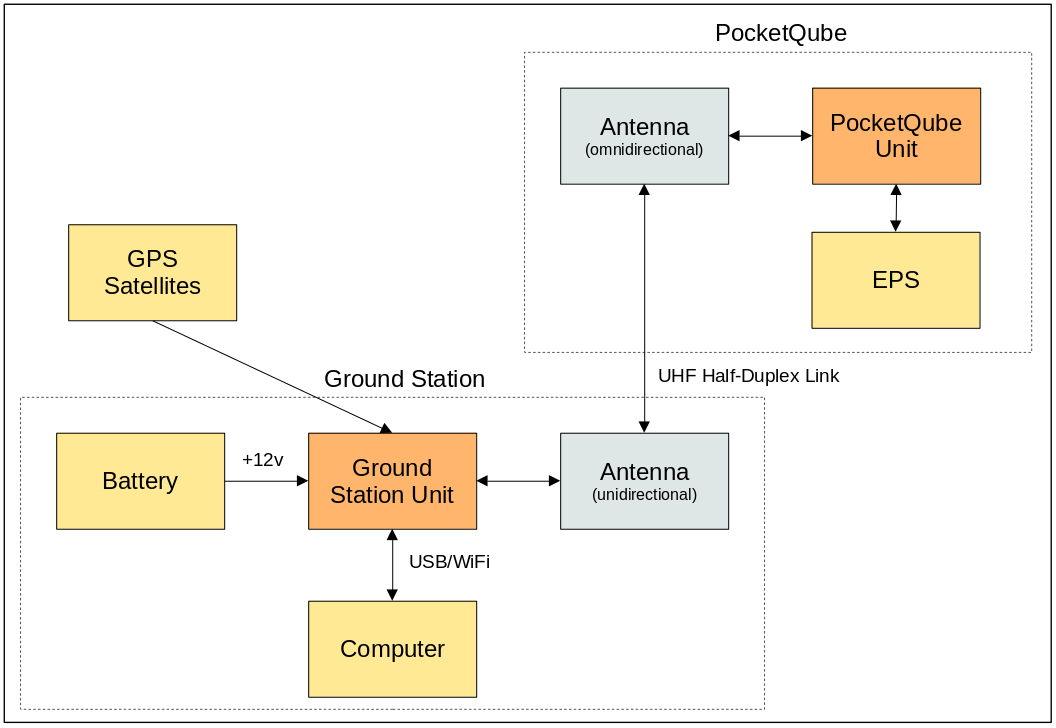
\includegraphics[width=0.65\textwidth]{complete_system.png}
    \caption{High-Level System Diagram}
    \label{fig:complete_system}
  \end{figure}

\subsection{Methodology}
Since a large number of sub-systems are required on the ground-station, either IC \textit{modules} or simple \textit{reference designs} will be form the basic building blocks of the system. Only if no modules or designs are found to meet the system requirements, will a more custom solution be developed. The ground station will be powered via +12V from a nearby vehicle, and the PocketQube will be powered from an on-board EPS (another PQ unit). Both sub-systems should be designed such that testing without a vehicle/EPS is also possible.

\subsection{Tracking}
Further research shows that trajectory predictions for both the landing area and the dynamic altitude of a balloon can be up to 15-20 km inaccurate for a standard 2 hour flight \cite{paper-balloonTrajectoryAnalysis}. For the worst case, this is a total inaccuracy of $\sqrt{20^2 + 20^2} = \SI{28}{km}$. For the designed range of 120 km, this results in an angle inaccuracy of $360 \times \frac{28}{2 \pi \times 120} \approx 14^\circ$.

An antenna with a beamwidth of double this inaccuracy is therefore required. A Yagi-Uda antenna with a beamwidth of around $28^\circ$ has a gain of around 17 dBi, as seen in Figure \ref{fig:antennaGain}. Using a common Si4311 FSK receiver's sensitivity of -104 dBm, an initial link budget can be estimated. Assuming 100 mW (20 dB) transmit power, the full 22 dBi gain, and 127 dB path loss attenuation loss at 115 km, a 10 dB link margin is obtained.

Since the above link budget clearly indicates that open-loop tracking is feasible, it is decided to focus on this as the main tracking method. The ground station therefore requires at least a GPS connection; a means of determining true north (such as a magnetometer); and a means of uploading path data. The path data will be uploaded to the ground station via USB from a system computer. If time allows, direct GPS tracking will then be added as a method of "closing the loop", and to improve pointing accuracy.

\subsection{Custom Link}
A half-duplex link will be designed. This is decided on due to the nature of the link itself (i.e. either downlink ``telemetry" or a simple command-response ``telecommand" pattern) and due to the added complexity that full-duplex would require (i.e. a duel frequency system).

For the given flight path, a goal of at least 9600 downlink baud rate will be designed for at the 120 km range, with LoRa being explored as the main modulation technique. This is chosen due to the high sensitivity it offers (which will help alleviate the need for a large, high-gain antenna), as while as the link speed it offers a for reasonable bandwidth ($< \SI{500}{kHz}$). GFSK will be considered as a backup option, since it is well-established in literature. The 433 MHz amateur band (430 to 440 MHz) will be utilized.